\section{交换环论}

本节所论环均为交换含幺环, 环同态均保幺.

\subsection{概形}

\subsubsection{大根小根}

\begin{definition}
    记环 \(A\) 的全体素理想为素谱 \(\mathrm{Spec} (A)\), 全体极大理想为 \(\mathrm{MaxSpec} (A)\)
\end{definition}

\begin{definition}
    对 \(A\) 中理想 \(\mathfrak{a}\), 定义其根式理想 \(\sqrt{\mathfrak{a}} := \{a \in A : \exists n \in \mathbb{Z}_{>0} (a^n \in \mathfrak{a})\}\).

    \begin{proof}
        需证明其对加法乘法封闭, 对于 \(a,b \in \sqrt{\mathfrak{a}}\), 故有正整数 \(n,m\) 使得 \(a^n,b^m \in \mathfrak{a}\),
        从而 \((a+b)^(m+n) \in \mathfrak{a}\), 故 \(a + b \in \sqrt{\mathfrak{a}}\).

        对于 \(a \in \sqrt{\mathfrak{a}}\), 有正整数 \(n\) 是的 \(a^n \subseteq \mathfrak{a}\),
        故 \((a A)^n = a^n A^n \subseteq \mathfrak{a}\).
    \end{proof}
\end{definition}

\begin{lemma}
    小根 \(\sqrt{\{0\}} = \bigcap \mathrm{Spec} A\).

    \begin{proof}
        显然所有素理想均包含 \(\sqrt{\{0\}}\), 反之, 假设存在 \(x \neq \sqrt{\{0\}}\),
        可以构造不含 \(x\) 的极大的理想 \(\mathfrak{m}\), 需证明其素. 任取 \(a,b \notin \mathfrak{m}\),
        有 \(x \in \left\langle a \right\rangle + \mathfrak{m} \land x \in \left\langle b \right\rangle + \mathfrak{m}\),
        于是必然存在 \(\mu,\nu \in A,\alpha,\beta \in \mathfrak{m}\) 满足 \(x = \mu a + \alpha = \nu b + \beta\),
        于是 \(x = \mu \nu (a b) + (\alpha \beta + \alpha \nu b + \beta \mu a) \in \left\langle ab\right\rangle + \mathfrak{m}\),
        故 \(ab \notin \mathfrak{m}\).
    \end{proof}
\end{lemma}

\begin{definition}
    若 \(\sqrt{\{0\}} = 0\) 则称为约化环.
\end{definition}

\begin{corollary}
    全体包含 \(\mathfrak{a}\) 的素理想之交给出了 \(\sqrt{\mathfrak{a}}\).

    \begin{proof}
        对 \(A / \mathfrak{a}\) 应用上述结论.
    \end{proof}
\end{corollary}

\begin{lemma}
    \(x \in \bigcap \mathrm{MaxSpec} A\) 当且仅当 \(\forall y \in A \exists u \in A (u(1-xy) = 1)\).

    \begin{proof}
        若 \(x \notin \mathrm{MaxSpec} A\), 则有极大理想 \(\mathfrak{m}\) 使得 \(x \notin \mathfrak{m}\),
        于是存在 \(y \in {(x + \mathfrak{m})}^{-1} \in A / \mathfrak{m}\), 故 \(1 - xy \in \mathfrak{m}\) 不可逆.

        反之, 给定 \(y\) 且 \(1 - xy\) 不可逆, 则存在极大理想 \(\mathfrak{m}\) 使得 \(1 - xy \in \mathfrak{m}\),
        又 \(1 \notin \mathfrak{m}\) 故 \(x \notin \mathfrak{m}\).
    \end{proof}
\end{lemma}

\begin{definition}[理想除法]
    对理想 \(\mathfrak{a},\mathfrak{b}\), 定义理想 \((\mathfrak{a} : \mathfrak{b}) := \{x \in A : x \mathfrak{b} \subseteq \mathfrak{a}\}\).

    \begin{proof}
        对加法乘法的封闭性是显然的.
    \end{proof}
\end{definition}

\begin{lemma}
    有公式:

    \[
        \begin{aligned}
            \mathfrak{a} \subseteq (\mathfrak{a} : \mathfrak{b}) \\
            (\mathfrak{a} : \mathfrak{b}) \mathfrak{b} \subseteq \mathfrak{a} \\
            ((\mathfrak{a} : \mathfrak{b}) : \mathfrak{c}) = (\mathfrak{a} : \mathfrak{b} \mathfrak{c}) = ((\mathfrak{a} : \mathfrak{c}) : \mathfrak{b}) \\
            (\bigcap_i \mathfrak{a_i} : \mathfrak{b}) = \bigcap_i (\mathfrak{a_i} : \mathfrak{b}) \\
            (\mathfrak{a} : \sum_i \mathfrak{b}_i) = \bigcap_i (\mathfrak{a} : \mathfrak{b}_i)
        \end{aligned}
    \]

    \begin{proof}
        无非是集合上的验证.
    \end{proof}
\end{lemma}

\begin{lemma}
    有公式:

    \[
        \begin{aligned}
            \sqrt{\mathfrak{a}} \supseteq \mathfrak{a} \\
            \sqrt{\sqrt{\mathfrak{a}}} = \sqrt{\mathfrak{a}} \\
            \sqrt{\mathfrak{a} \mathfrak{b}} = \sqrt{\mathfrak{a} \cap \mathfrak{b}} = \sqrt{\mathfrak{a}} \cap \sqrt{\mathfrak{b}} \\
            \sqrt{\mathfrak{a} + \mathfrak{b}} = \sqrt{\sqrt{\mathfrak{a}} + \sqrt{\mathfrak{b}}} \\
            \mathfrak{p} \in \mathrm{Spec} A \implies \sqrt{\mathfrak{p}^n} = \mathfrak{p}
        \end{aligned}
    \]
\end{lemma}

\begin{lemma}
    给出素理想 \(\mathfrak{p}_1,\mathfrak{p}_2,\cdots, \mathfrak{p}_n\), 若 \(\mathfrak{a} \subseteq \bigcup_i \mathfrak{p}_i\),
    则 \(\exists i (\mathfrak{a} \subseteq \mathfrak{p}_i)\).

    \begin{proof}
        对 \(n\) 进行归纳, \(n = 1\) 时显然, 若对 \(n = k\) 成立, \(n = k+1\) 时,
        对某个 \(i\), 若不存在 \(x_i\) 使得 \(i \neq j \implies x_i \notin \mathfrak{p}_j\), 则被除 \(\mathfrak{p}_i\) 对素理想覆盖,
        依归纳假设成立, 故存在上述 \(x_i\), 考察互不相同的 \(x_i\) 的 \(n-1\) 项积, 共有 \(n\) 项, 求和, 知和不再任意一个 \(\mathfrak{p}_i\) 中.
    \end{proof}
\end{lemma}

\begin{lemma}
    给出素理想 \(\mathfrak{p}\) 以及理想 \(\mathfrak{a}_1,\mathfrak{a}_1, \cdots, \mathfrak{a}_n\), 若 \(\bigcap \mathfrak{a}_i \subseteq \mathfrak{p}\),
    则有 \(i\) 使得 \(\mathfrak{a}_i \subseteq \mathfrak{p}\).

    \begin{proof}
        若否, 则每个 \(\mathfrak{a}_i\) 中均存在 \(\alpha_i \notin \mathfrak{p}\),
        则 \(\prod_i \alpha_i \in \bigcap_i \mathfrak{a}_i\) 满足 \(\prod_i \alpha_i \notin \bigcap_i \mathfrak{p}\).
    \end{proof}
\end{lemma}

\begin{lemma}
    给出素理想 \(\mathfrak{p}\) 以及理想 \(\mathfrak{a}_i\), 若 \(\mathfrak{p} = \bigcap \mathfrak{a}_i\), 则有 \(i\) 使得 \(\mathfrak{p} = \mathfrak{a}_i\).

    \begin{proof}
        考察 \(A / \mathfrak{a}\), 必然有一项包含 \(1\) 的理想.
    \end{proof}
\end{lemma}

\subsubsection{Zariski 拓扑}

\begin{definition}
    \label {definition:Zariski topology}
    在 \(\mathrm{Spec} (A)\) 上定义闭集为 \(\{V(S) := \{\mathfrak{p} \in \mathrm{Spec} (A) : S \subseteq \mathfrak{p}\} : S \subseteq A\}\),
    称为 Zariski 拓扑.

    \begin{proof}
        需证明其对无限交, 有限并封闭, 只需注意到 \(\bigcap_i V(S_i) = V(\bigcup_i S_i)\), \(V(S_1) \cup V(S_2) = V(S_1 S_2)\),
        其中 \(S_1 S_2 := \{ab : a \in S_1, b \in S_2\}\).
    \end{proof}
\end{definition}

\begin{lemma}
    \(A\) 的根式理想与 Zariski 拓扑的闭集一一对应.

    \begin{proof}
        素理想的交即为根式理想.
    \end{proof}
\end{lemma}

\begin{corollary}
    Zariski 拓扑带有自然的拓扑基 \(\{D(f) := \mathrm{Spec} (A) \setminus V(\{f\}) : f \in A\}\).
\end{corollary}

\begin{lemma}
    Zariski 拓扑总是 \ref{definition:compact topological space} 的.

    \begin{proof}
        假定 \(V(\{f_i\})\) 交为 \(0\), 也即不存在含全体 \(f_i\) 的极大理想, 故给出 \(1 = \sum_{j=1}^{n} a_{i_j} f_{i_j}\),
        找出求和式对应的 \(f_{i_j}\) 即可.
    \end{proof}
\end{lemma}

\begin{lemma}
    \(A = \prod_i A_i\) 时, \(\mathrm{Spec} (A) = \coprod_i \mathrm{Spec} (A_i)\).

    \begin{proof}
        注意到 \(A\) 的素理想均为形如 \(\pi_i^{-1} (\mathfrak{p}_i)\) 的理想,
        而闭集均为 \(V(S) = \coprod_i V(\pi_i (S))\).
    \end{proof}
\end{lemma}

\begin{lemma}
    若 \(\mathrm{Spec} (A)\) 不连通, 则 \(A = A_1 \times A_2\), 其中 \(A_1,A_2\) 非平凡.

    \begin{proof}
        给出 \(I,J\) 即开又闭且覆盖 \(\mathrm{Spec} A\), 对应有理想 \(\mathfrak{m} = \bigcap I, \mathfrak{n} = \bigcap J\),
        注意到 \(I \cap J = \varnothing\), 故有 \(\mathfrak{m} + \mathfrak{n} = A\), 于是有 \(m \in \mathfrak{m}, n \in \mathfrak{n}\) 使得 \(m + n = 1\),
        而 \(mn \in \mathfrak{m} \cap \mathfrak{n} \in \bigcap \mathrm{Spec} A\), 故存在 \(k\) 使得 \(m^k n^k = 0\), 于是给出了 \(\alpha := \sum_{i=0}^{k-1} \binom{2k-1}{i} m^{2k-i-1} n^{i}, \beta := \sum_{i=k}^{2k-1} \binom{2k-1}{i} m^{2k-i-1} n^{i}\),
        满足 \(\alpha + \beta = 1\), 且 \(\alpha \beta = 0\), 于是 \(A = \alpha A \times \beta A\).
    \end{proof}
\end{lemma}

\begin{lemma}
    环同态 \(\varphi : A \to B\) 诱导了连续映射 \(\varphi^\ast : \mathrm{Spec} (B) \to \mathrm{Spec} (A)\).

    \begin{proof}
        对应理想的拉回 \(\mathfrak{p} \mapsto \varphi^{-1}(\mathfrak{p})\), 连续性只需注意到闭集 \(\{V(S) : S \subseteq A\}\) 在诱导出的 \(\mathrm{Spec} (B) \to \mathrm{Spec} (A)\) 下的拉回为 \(\{V(\varphi(S)) : S \subseteq A\}\).
    \end{proof}
\end{lemma}

\begin{lemma}
    \label {lemma:irreducible iff domain}
    \(\mathrm{Spec} (A)\) \ref{definition:irreducible topological space} 当且仅当 \(A\) 是整环.

    \begin{proof}
        \(\implies\): 假定 \(ab = 0\), 则 \(V(\{a\}) \cup V(\{b\}) = V(\{0\}) = \mathrm{Spec} (A)\).

        \(\impliedby\): 若 \(A\) 是整环, 则有一般点 \(\{0\}\).
    \end{proof}
\end{lemma}

\begin{remark}
    我们称元素 \(f\) 在 \(\mathfrak{p} \in \mathrm{Spec} (A)\) 的值为 \(f \mathfrak{p} \in A / \mathfrak{p}\).
\end{remark}

\begin{remark}
    闭集诱导 \(f(\mathfrak{p}) = 0\), 也即闭集对应方程, 而开集则对应坐标系.
\end{remark}

\subsubsection{局部化}

局部化的操作是隐去某个闭集而只考虑其余的开集, 闭集对应方程, 我们将对应的方程做分母, 即可排除这些点.

\begin{definition}[局部化]
    对于一个乘性子集 \(S \subseteq A\), 即满足 \(1 \in S\) 且 \(S\) 对乘法封闭, 定义局部化 \(S^{-1} A\) 为 \(A \times S / \{((a,s),(a^\prime,s^\prime)) \in (A \times S) \times (A \times S) : \exists t \in S ((a s^\prime - a^\prime s) t = 0)\}\), 
    用 \(\frac{a}{s}\) 记 \((a,s)\) 其赋予环结构如下:

    \[
        \begin{aligned}
            \frac{a}{s} + \frac{a^\prime}{s^\prime} &:= \frac{a s^\prime + a^\prime s}{s s^\prime} \\
            \frac{a}{s} \cdot \frac{a^\prime}{s^\prime} &:= \frac{a a^\prime}{s s^\prime}
        \end{aligned}
    \]
\end{definition}

\begin{example}
    对于非幂零 \(f \in A\), 给出乘性子集 \(\{f^n : n \in \mathbb{N}\}\), 记对其的局部化为 \(A_f\).
\end{example}

\begin{example}
    对于素理想 \(\mathfrak{p}\), 给出乘性子集 \(A \setminus \mathfrak{p}\), 记对其的局部化为 \(A_{\mathfrak{p}}\).
\end{example}

\begin{lemma}[局部化的泛性质]
    对于任意同态 \(A \to B\) 以及乘性子集 \(S \subseteq A\), 若 \(\phi (S) \subseteq B^{\times}\) 均可逆,
    则存在唯一的同态 \(S^{-1} A \to B\) 使得下图交换:

    \begin{center}
        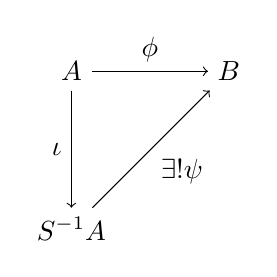
\begin{tikzpicture}
            \node (A) at (0,0) {\(A\)};
            \node (B) at (2,0) {\(B\)};
            \node (S) at (0,-2) {\(S^{-1} A\)};

            \draw [->] (A) to node [above] {\(\phi\)} (B);
            \draw [->] (A) to node [left] {\(\iota\)} (S);
            \draw [->] (S) to node [below right] {\(\exists !\psi\)} (B);
        \end{tikzpicture}
    \end{center}
\end{lemma}

\begin{lemma}
    局部化和商交换, 令 \(\overline{S} = S I\), 则有自然同构 \((S^{-1} A / I S^{-1} A) \cong \overline{S}^{-1} (A / I)\),
    当然这里要求 \(I \cap S = \varnothing\).

    \begin{proof}
        验证泛性质, 考察全体 \(A \to B\) 使得 \(I\) 映为 \(0\), \(S\) 可逆.
    \end{proof}
\end{lemma}

\begin{corollary}
    有域同构 \(\mathrm{Frac} (A / \mathfrak{p}) \cong A_{\mathfrak{p}} / \mathfrak{p} A_{\mathfrak{p}}\).
\end{corollary}

\begin{lemma}
    对乘性子集 \(S_1,S_2\) 定义 \(S_1 S_2 := \{s_1 s_2 : s_1 \in S_1, s_2 \in S_2\}\), 则有自然同构 \({S_1}^{-1} ({S_2}^{-1} A) \cong {(S_1 S_2)}^{-1} A\).
\end{lemma}

\begin{lemma}
    有同构 \(S^{-1} (A[X]) \cong (S^{-1} A)[X]\), 也即局部化和多项式交换.
\end{lemma}

\begin{lemma}
    嵌入 \(A \to S^{-1} A\) 诱导出 \(\mathrm{Spec} (S^{-1} A) \to \{\mathfrak{p} \in \mathrm{Spec} (A) : S \cap \mathfrak{p} = \varnothing\}\) 的同胚.

    \begin{proof}
        有同构 \(S^{-1} A / \mathfrak{p} S^{-1} A \cong \overline{S}^{-1} (A / \mathfrak{p})\) 其保持零点故给出双射 \(\mathfrak{q} \mapsto \mathfrak{q} \cap A, \mathfrak{p} \mapsto \mathfrak{p} S^{-1} A\) 为同胚.
    \end{proof}
\end{lemma}

\begin{lemma}
    对于点 \(f\), 理想 \(I\), 有同胚 \(\mathrm{Spec} (A_f) \to D(f)\), \(\mathrm{Spec} (A / I) \to V(I)\).

    \begin{proof}
        第一个论断即上述引理, 同构 \(A/I/\mathfrak{p} = A/\mathfrak{p}/I\) 给出 \(A \to A/I\) 对应的 \(\mathrm{Spec} (A/I) \to V(f) \subseteq \mathrm{Spec} (A)\) 双射为同胚.
    \end{proof}
\end{lemma}

\begin{lemma}
    环同态 \(\varphi : A \to B\) 在素谱空间 \(\varphi^\ast : \mathrm{Spec} (B) \to \mathrm{Spec} (A)\) 的 \(\mathfrak{p} \in \mathrm{Spec} (A)\) 处纤维 \({\varphi^{\ast}}^{-1} (\{\mathfrak{p}\})\) 为 \(\mathrm{Spec} (B_{\phi(A \setminus \mathfrak{p})}/\varphi(\mathfrak{p}) B_{\phi(A \setminus \mathfrak{p})})\).

    \begin{proof}
        要求素理想不交 \(\varphi(A \setminus \mathfrak{p})\) 且包含 \(\varphi(\mathfrak{p})\) 即上述 \(\mathrm{Spec}\).
    \end{proof}
\end{lemma}

\begin{example}
    考察 \(A\) 的代数扩张 \(A[X] / (f)\), 对 \(A\) 的素理想 \(\mathfrak{p}\), 注意到有等式:

    \[
        \frac{(A[X]/(f))_{A \setminus \mathfrak{p}}}{\mathfrak{p} (A[X]/(f))_{A \setminus \mathfrak{p}}} = {(\frac{(A[X]/(f))}{\mathfrak{p} (A[X]/(f))})}_{A \setminus \mathfrak{p}}
        = {(\frac{(A/\mathfrak{p}) [X]}{(f)})}_{A \setminus \mathfrak{p}} = \frac{\mathrm{Frac} (A / \mathfrak{p})[X]}{(f)}
    \]

    所以 \(\mathfrak{p}\) 的纤维为 \(\mathrm{Spec} (\frac{\mathrm{Frac} (A / \mathfrak{p})[X]}{(f)})\), 以 \(\mathbb{Z} [X] / (X^2 + 1)\) 为例, 只需考察 \(\mathbb{F}_p [X]\) 中 \(X^2 + 1\) 的分解即可.
\end{example}

\begin{corollary}
    \(V(I)\) 不可约当且仅当 \(\sqrt{I}\) 是素理想.

    \begin{proof}
        利用 \(\mathrm{Spec} (A/I) \cong V(I)\) 与 \ref{lemma:irreducible iff domain} 即可.
    \end{proof}
\end{corollary}
